%!TEX root =../mapp-challenge-18-game-book.tex
% ^ leave for LaTeXTools build functionality

\begin{wrapfigure}{r}{0.33\textwidth} %this figure will be at the right
    \centering
      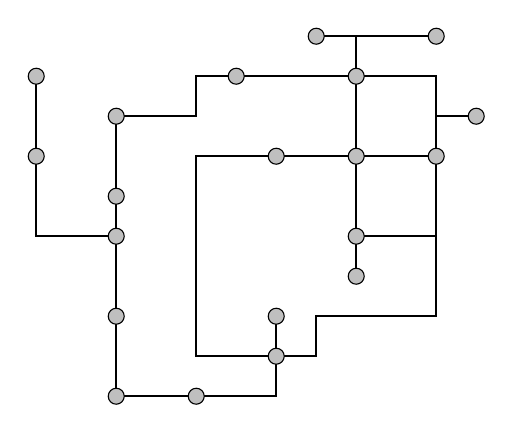
\begin{tikzpicture}[x=0.2in,y=0.2in,every node/.style={circle,fill=lightgray,
                          draw=black,text width=1em,align=center}]
        \draw[thick] (2,0) -- (2,7) -- (4,7) -- (4,8) -- (10,8) --
              (10,2) -- (7,2) -- (7,1) -- (6,1) -- (6,0) -- (2,0);
        \draw[thick] (8,9) -- (8,3);
        \draw[thick] (8,4) -- (10,4);
        \draw[thick] (7,9) -- (10,9);
        \draw[thick] (10,6) -- (4,6) -- (4,1) -- (6,1);
        \draw[thick] (10,7) -- (11,7);
        \draw[thick] (2,4) -- (0,4) -- (0,8);
        \draw[thick] (6,1) -- (6,2);

        \draw[fill=lightgray,draw=black] (2,2) circle (0.2);
        \draw[fill=lightgray,draw=black] (2,4) circle (0.2);
        \draw[fill=lightgray,draw=black] (2,5) circle (0.2);
        \draw[fill=lightgray,draw=black] (2,7) circle (0.2);
        \draw[fill=lightgray,draw=black] (5,8) circle (0.2);
        \draw[fill=lightgray,draw=black] (8,8) circle (0.2);
        \draw[fill=lightgray,draw=black] (10,9) circle (0.2);
        \draw[fill=lightgray,draw=black] (8,4) circle (0.2);
        \draw[fill=lightgray,draw=black] (8,3) circle (0.2);
        \draw[fill=lightgray,draw=black] (10,6) circle (0.2);
        \draw[fill=lightgray,draw=black] (6,6) circle (0.2);
        \draw[fill=lightgray,draw=black] (8,6) circle (0.2);
        \draw[fill=lightgray,draw=black] (6,1) circle (0.2);
        \draw[fill=lightgray,draw=black] (6,2) circle (0.2);
        \draw[fill=lightgray,draw=black] (4,0) circle (0.2);
        \draw[fill=lightgray,draw=black] (2,0) circle (0.2);
        \draw[fill=lightgray,draw=black] (11,7) circle (0.2);
        \draw[fill=lightgray,draw=black] (0,6) circle (0.2);
        \draw[fill=lightgray,draw=black] (0,8) circle (0.2);
        \draw[fill=lightgray,draw=black] (7,9) circle (0.2);
      \end{tikzpicture}
\end{wrapfigure}

Welcome to the world of \textbf{Mobile Monsters}, or \textbf{\mappMobimon}
for short! Not to be confused with the similarly named video game series loved
by fans the world over, \mappMobimon{} is a \textit{completely original} concept
where Trainers befriend monsters and use them to battle opponents. (Cough.)

Under the guidance of your mentor, \textbf{Dr. Treename}, you will soon set off
on your adventure to befriend the \mappMobimon{} of the \textbf{Kantor region}.
You'll meet many strange characters, but if you can solve their problems
they just might lead you to the location of the \textbf{Dojo Masters}.
By earning their respect, you'll be allowed to enter the
\textbf{\mappMobimon{} Tournament} for the chance to be crowned
\textbf{\mappMobimon{} Champion}! Maybe you'll even discover the location
of the Legendary \mappMobimon{} \(\mu\)Too?...

As you might expect, most of the challenges you'll face today won't actually
be combat related. In the world of \mappMobimon{}, nothing is more important
than your \textbf{problem-solving abilities}. So sharpen your minds and
pencils, because you never know when a wild \textbf{puzzle} will appear!


%%% Local Variables:
%%% mode: latex
%%% TeX-master: "../mapp-hsc17-game-book"
%%% End:
